% =============================================================================
% Dissertation/manuscript.tex — top-level monograph assembly
%
% Compile from inside this directory (3-pass XeLaTeX + bibtex):
%   TEXINPUTS=../Preambles:$TEXINPUTS xelatex -interaction=nonstopmode manuscript.tex
%   BIBINPUTS=..:$BIBINPUTS bibtex manuscript
%   TEXINPUTS=../Preambles:$TEXINPUTS xelatex -interaction=nonstopmode manuscript.tex  (x2)
%
% STRUCTURE. This is a monograph, not a 3-paper collection. Chapters live in
% chapters/ and are pulled in with \include{} (each \include starts a new
% page and lets us compile a single chapter with \includeonly during drafting).
%
% SINGLE SOURCE OF TRUTH. This manuscript is authoritative. Every numeric claim
% must trace back to the R pipelines under analyses/NN/ via:
%   - \input{tables/<name>.tex}          for regression tables
%   - %% source: analyses/01_quant_main/scripts/R/03_analyze.R   for inline numbers
% so /audit-reproducibility can verify them across the paper<->code graph.
% =============================================================================

\documentclass[12pt]{report}

% Shared dissertation preamble (palette, packages, math, hyperref).
% Found via TEXINPUTS=../Preambles; see Preambles/header.tex.
\input{header}

% --- Monograph-specific packages --------------------------------------------
\usepackage{geometry}
\geometry{margin=1in}
\usepackage{setspace}
\doublespacing

% --- Figure paths (relative to this file) -----------------------------------
% Chapters \includegraphics figures from Dissertation/figures/. Analyses write
% their finished PDFs there; \input{} table fragments come from Dissertation/tables/.
\graphicspath{{figures/}}

% --- Front matter -----------------------------------------------------------
\title{US--China Aid Competition in the 21st Century:\\
       \large Aid Races across Spheres of Influence}
\author{Hasaan Parker \\ \small{Department of Political Science, University of Wisconsin--Madison}}
\date{\today}

% During drafting, uncomment and list the chapter(s) you want to compile fast:
% \includeonly{chapters/ch04_quant_main}

\begin{document}

\maketitle

\begin{abstract}
\noindent
\textit{Abstract placeholder.} A single-argument statement of the dissertation:
the question (how does US--China donor competition reshape aid allocation
across contested spheres of influence?), the theory (aid races vs.\ aid
withdrawal), the empirical strategy (short-run allocation models plus a
long-run dynamics test), and the headline finding (a positive US--China aid
correlation in Africa, negative elsewhere). Aim for 150--250 words once written.
\end{abstract}

\tableofcontents

% =============================================================================
% Chapters. Each file begins with \chapter{...}. Fill over time; the argument
% is a single through-line, not three separable papers.
% =============================================================================
% =============================================================================
% chapters/ch01_intro.tex — Introduction
% Pulled into manuscript.tex via % =============================================================================
% chapters/ch01_intro.tex — Introduction
% Pulled into manuscript.tex via % =============================================================================
% chapters/ch01_intro.tex — Introduction
% Pulled into manuscript.tex via \include{chapters/ch01_intro}.
% =============================================================================
\chapter{Introduction}
\label{ch:intro}

\textit{Placeholder.} Motivate the puzzle: as China has scaled up development
finance across the Global South, does US aid respond by \emph{racing} (matching
Chinese entry to hold a sphere of influence) or by \emph{withdrawing} (ceding
contested recipients)? State the dissertation's single argument, its
contribution to the foreign-aid-competition literature, and the roadmap through
the chapters that follow.

\section{The puzzle}
\textit{Placeholder.} Great-power competition and the return of aid as
statecraft.

\section{Argument in brief}
\textit{Placeholder.} Aid races vs.\ aid withdrawal, conditioned by whether a
recipient sits inside a contested sphere of influence.

\section{Contribution}
\textit{Placeholder.} What this monograph adds over existing work on donor
competition and recipient strategy.

\section{Roadmap}
\textit{Placeholder.} Chapter~\ref{ch:lit} reviews the literature;
Chapter~\ref{ch:theory} develops the theory and hypotheses;
Chapter~\ref{ch:quant} presents the quantitative evidence;
Chapter~\ref{ch:conclusion} concludes.
.
% =============================================================================
\chapter{Introduction}
\label{ch:intro}

\textit{Placeholder.} Motivate the puzzle: as China has scaled up development
finance across the Global South, does US aid respond by \emph{racing} (matching
Chinese entry to hold a sphere of influence) or by \emph{withdrawing} (ceding
contested recipients)? State the dissertation's single argument, its
contribution to the foreign-aid-competition literature, and the roadmap through
the chapters that follow.

\section{The puzzle}
\textit{Placeholder.} Great-power competition and the return of aid as
statecraft.

\section{Argument in brief}
\textit{Placeholder.} Aid races vs.\ aid withdrawal, conditioned by whether a
recipient sits inside a contested sphere of influence.

\section{Contribution}
\textit{Placeholder.} What this monograph adds over existing work on donor
competition and recipient strategy.

\section{Roadmap}
\textit{Placeholder.} Chapter~\ref{ch:lit} reviews the literature;
Chapter~\ref{ch:theory} develops the theory and hypotheses;
Chapter~\ref{ch:quant} presents the quantitative evidence;
Chapter~\ref{ch:conclusion} concludes.
.
% =============================================================================
\chapter{Introduction}
\label{ch:intro}

\textit{Placeholder.} Motivate the puzzle: as China has scaled up development
finance across the Global South, does US aid respond by \emph{racing} (matching
Chinese entry to hold a sphere of influence) or by \emph{withdrawing} (ceding
contested recipients)? State the dissertation's single argument, its
contribution to the foreign-aid-competition literature, and the roadmap through
the chapters that follow.

\section{The puzzle}
\textit{Placeholder.} Great-power competition and the return of aid as
statecraft.

\section{Argument in brief}
\textit{Placeholder.} Aid races vs.\ aid withdrawal, conditioned by whether a
recipient sits inside a contested sphere of influence.

\section{Contribution}
\textit{Placeholder.} What this monograph adds over existing work on donor
competition and recipient strategy.

\section{Roadmap}
\textit{Placeholder.} Chapter~\ref{ch:lit} reviews the literature;
Chapter~\ref{ch:theory} develops the theory and hypotheses;
Chapter~\ref{ch:quant} presents the quantitative evidence;
Chapter~\ref{ch:conclusion} concludes.

% =============================================================================
% chapters/ch02_lit.tex — Related Literature
% Pulled into manuscript.tex via % =============================================================================
% chapters/ch02_lit.tex — Related Literature
% Pulled into manuscript.tex via % =============================================================================
% chapters/ch02_lit.tex — Related Literature
% Pulled into manuscript.tex via \include{chapters/ch02_lit}.
% =============================================================================
\chapter{Related Literature}
\label{ch:lit}

\textit{Placeholder.} Position the dissertation relative to three literatures:
(i) the political economy of foreign aid allocation; (ii) US--China strategic
competition and aid as statecraft; and (iii) recipient-side agency and donor
coordination. Identify the gap the monograph fills.

\section{The political economy of aid allocation}
\textit{Placeholder.} Donor interests vs.\ recipient need; the strategic-aid
tradition.

\section{China as a development donor}
\textit{Placeholder.} AidData GCDF-based work on Chinese official finance;
comparisons to OECD-DAC donors.

\section{Aid competition and spheres of influence}
\textit{Placeholder.} Existing accounts of donor rivalry and what ``sphere of
influence'' has meant empirically. Motivates the operationalization refined in
Chapter~\ref{ch:theory}.
.
% =============================================================================
\chapter{Related Literature}
\label{ch:lit}

\textit{Placeholder.} Position the dissertation relative to three literatures:
(i) the political economy of foreign aid allocation; (ii) US--China strategic
competition and aid as statecraft; and (iii) recipient-side agency and donor
coordination. Identify the gap the monograph fills.

\section{The political economy of aid allocation}
\textit{Placeholder.} Donor interests vs.\ recipient need; the strategic-aid
tradition.

\section{China as a development donor}
\textit{Placeholder.} AidData GCDF-based work on Chinese official finance;
comparisons to OECD-DAC donors.

\section{Aid competition and spheres of influence}
\textit{Placeholder.} Existing accounts of donor rivalry and what ``sphere of
influence'' has meant empirically. Motivates the operationalization refined in
Chapter~\ref{ch:theory}.
.
% =============================================================================
\chapter{Related Literature}
\label{ch:lit}

\textit{Placeholder.} Position the dissertation relative to three literatures:
(i) the political economy of foreign aid allocation; (ii) US--China strategic
competition and aid as statecraft; and (iii) recipient-side agency and donor
coordination. Identify the gap the monograph fills.

\section{The political economy of aid allocation}
\textit{Placeholder.} Donor interests vs.\ recipient need; the strategic-aid
tradition.

\section{China as a development donor}
\textit{Placeholder.} AidData GCDF-based work on Chinese official finance;
comparisons to OECD-DAC donors.

\section{Aid competition and spheres of influence}
\textit{Placeholder.} Existing accounts of donor rivalry and what ``sphere of
influence'' has meant empirically. Motivates the operationalization refined in
Chapter~\ref{ch:theory}.

% =============================================================================
% chapters/ch03_theory.tex — Theory & Hypotheses
% Pulled into manuscript.tex via % =============================================================================
% chapters/ch03_theory.tex — Theory & Hypotheses
% Pulled into manuscript.tex via % =============================================================================
% chapters/ch03_theory.tex — Theory & Hypotheses
% Pulled into manuscript.tex via \include{chapters/ch03_theory}.
% =============================================================================
\chapter{Theory: Aid Races and Aid Withdrawal}
\label{ch:theory}

\textit{Placeholder.} Develop the core theory: when a donor faces a strategic
rival entering a recipient it values, it either escalates (an \emph{aid race})
or disengages (\emph{aid withdrawal}). Which response dominates depends on
whether the recipient lies within a contested sphere of influence and on the
type of good the aid delivers.

\section{Spheres of influence, operationalized}
\label{sec:soi-operational}
The first-pass operationalization used continent as a stand-in for ``sphere of
influence.'' That was always a coarse proxy -- continent doesn't distinguish a
country firmly in the US camp from a genuinely contested neighbor -- and
Chapter~\ref{ch:quant} shows the region cut produces a diffuse, largely
non-significant pattern once standard errors are handled correctly. The
refined operationalization (voting-alignment component only; geographic
proximity and historical-ties components are not yet built) uses each
country's UN General Assembly ideal point (Voeten, Sep.\ 2023 release) to
locate it relative to both powers:
\[
\text{rel\_align}_{i,t} = |\text{ideal}_{i,t} - \text{ideal}_{\text{CHN},t}| - |\text{ideal}_{i,t} - \text{ideal}_{\text{US},t}|
\]
Large positive values mean a country votes far from China and close to the US
(\emph{US-aligned}); large negative values mean the reverse (\emph{China-aligned});
values near zero mean the country is roughly equidistant --
genuinely \emph{contested}. Countries are terciled into these three blocs
\textbf{within year} (ideal-point scales are not necessarily comparable across
UNGA sessions) \textbf{and within the US-aid-recipient sample} (not the full
UN membership, so a bloc means ``relative to other aid recipients''), using
the bloc as of $t-1$ so this year's aid decision cannot
retroactively define the very bloc it is tested against. This SOI measure is
tested directly in Chapter~\ref{ch:quant}.

\section{H1: Aid races vs.\ aid withdrawal}
\textbf{H1.} In contested spheres, US and Chinese aid co-move positively (a
race); where the US has effectively already lost a recipient to China, US aid
falls as Chinese aid rises (withdrawal) -- a country already secured in the
US's own camp carries no sharp prediction either way. The prospectus finding
of $+0.113$ in Africa and negative correlations elsewhere was the original
motivating pattern; Chapter~\ref{ch:quant} tests this directly against the
alignment-based SOI blocs above, and the result is not what H1 predicts.

\section{H2: Private vs.\ public goods delivery}
\textit{Placeholder.} \textbf{H2.} The race is sharper where aid is delivered
as private/excludable goods (e.g., government-to-government projects) than where
it flows through NGOs to broad public goods. Tested in
\texttt{analyses/02\_h2\_private\_goods/}.
.
% =============================================================================
\chapter{Theory: Aid Races and Aid Withdrawal}
\label{ch:theory}

\textit{Placeholder.} Develop the core theory: when a donor faces a strategic
rival entering a recipient it values, it either escalates (an \emph{aid race})
or disengages (\emph{aid withdrawal}). Which response dominates depends on
whether the recipient lies within a contested sphere of influence and on the
type of good the aid delivers.

\section{Spheres of influence, operationalized}
\label{sec:soi-operational}
The first-pass operationalization used continent as a stand-in for ``sphere of
influence.'' That was always a coarse proxy -- continent doesn't distinguish a
country firmly in the US camp from a genuinely contested neighbor -- and
Chapter~\ref{ch:quant} shows the region cut produces a diffuse, largely
non-significant pattern once standard errors are handled correctly. The
refined operationalization (voting-alignment component only; geographic
proximity and historical-ties components are not yet built) uses each
country's UN General Assembly ideal point (Voeten, Sep.\ 2023 release) to
locate it relative to both powers:
\[
\text{rel\_align}_{i,t} = |\text{ideal}_{i,t} - \text{ideal}_{\text{CHN},t}| - |\text{ideal}_{i,t} - \text{ideal}_{\text{US},t}|
\]
Large positive values mean a country votes far from China and close to the US
(\emph{US-aligned}); large negative values mean the reverse (\emph{China-aligned});
values near zero mean the country is roughly equidistant --
genuinely \emph{contested}. Countries are terciled into these three blocs
\textbf{within year} (ideal-point scales are not necessarily comparable across
UNGA sessions) \textbf{and within the US-aid-recipient sample} (not the full
UN membership, so a bloc means ``relative to other aid recipients''), using
the bloc as of $t-1$ so this year's aid decision cannot
retroactively define the very bloc it is tested against. This SOI measure is
tested directly in Chapter~\ref{ch:quant}.

\section{H1: Aid races vs.\ aid withdrawal}
\textbf{H1.} In contested spheres, US and Chinese aid co-move positively (a
race); where the US has effectively already lost a recipient to China, US aid
falls as Chinese aid rises (withdrawal) -- a country already secured in the
US's own camp carries no sharp prediction either way. The prospectus finding
of $+0.113$ in Africa and negative correlations elsewhere was the original
motivating pattern; Chapter~\ref{ch:quant} tests this directly against the
alignment-based SOI blocs above, and the result is not what H1 predicts.

\section{H2: Private vs.\ public goods delivery}
\textit{Placeholder.} \textbf{H2.} The race is sharper where aid is delivered
as private/excludable goods (e.g., government-to-government projects) than where
it flows through NGOs to broad public goods. Tested in
\texttt{analyses/02\_h2\_private\_goods/}.
.
% =============================================================================
\chapter{Theory: Aid Races and Aid Withdrawal}
\label{ch:theory}

\textit{Placeholder.} Develop the core theory: when a donor faces a strategic
rival entering a recipient it values, it either escalates (an \emph{aid race})
or disengages (\emph{aid withdrawal}). Which response dominates depends on
whether the recipient lies within a contested sphere of influence and on the
type of good the aid delivers.

\section{Spheres of influence, operationalized}
\label{sec:soi-operational}
The first-pass operationalization used continent as a stand-in for ``sphere of
influence.'' That was always a coarse proxy -- continent doesn't distinguish a
country firmly in the US camp from a genuinely contested neighbor -- and
Chapter~\ref{ch:quant} shows the region cut produces a diffuse, largely
non-significant pattern once standard errors are handled correctly. The
refined operationalization (voting-alignment component only; geographic
proximity and historical-ties components are not yet built) uses each
country's UN General Assembly ideal point (Voeten, Sep.\ 2023 release) to
locate it relative to both powers:
\[
\text{rel\_align}_{i,t} = |\text{ideal}_{i,t} - \text{ideal}_{\text{CHN},t}| - |\text{ideal}_{i,t} - \text{ideal}_{\text{US},t}|
\]
Large positive values mean a country votes far from China and close to the US
(\emph{US-aligned}); large negative values mean the reverse (\emph{China-aligned});
values near zero mean the country is roughly equidistant --
genuinely \emph{contested}. Countries are terciled into these three blocs
\textbf{within year} (ideal-point scales are not necessarily comparable across
UNGA sessions) \textbf{and within the US-aid-recipient sample} (not the full
UN membership, so a bloc means ``relative to other aid recipients''), using
the bloc as of $t-1$ so this year's aid decision cannot
retroactively define the very bloc it is tested against. This SOI measure is
tested directly in Chapter~\ref{ch:quant}.

\section{H1: Aid races vs.\ aid withdrawal}
\textbf{H1.} In contested spheres, US and Chinese aid co-move positively (a
race); where the US has effectively already lost a recipient to China, US aid
falls as Chinese aid rises (withdrawal) -- a country already secured in the
US's own camp carries no sharp prediction either way. The prospectus finding
of $+0.113$ in Africa and negative correlations elsewhere was the original
motivating pattern; Chapter~\ref{ch:quant} tests this directly against the
alignment-based SOI blocs above, and the result is not what H1 predicts.

\section{H2: Private vs.\ public goods delivery}
\textit{Placeholder.} \textbf{H2.} The race is sharper where aid is delivered
as private/excludable goods (e.g., government-to-government projects) than where
it flows through NGOs to broad public goods. Tested in
\texttt{analyses/02\_h2\_private\_goods/}.

% =============================================================================
% chapters/ch04_quant_main.tex — Quantitative core (the empirical burden)
% Pulled into manuscript.tex via % =============================================================================
% chapters/ch04_quant_main.tex — Quantitative core (the empirical burden)
% Pulled into manuscript.tex via % =============================================================================
% chapters/ch04_quant_main.tex — Quantitative core (the empirical burden)
% Pulled into manuscript.tex via \include{chapters/ch04_quant_main}.
%
% This chapter carries the dissertation's empirical weight (the qualitative case
% chapters were dropped). Every number here must trace to an R pipeline under
% Dissertation/analyses/NN/. Wiring convention:
%   - Table fragments:  \input{tables/<name>.tex}
%     produced by analyses/01_quant_main/scripts/R/04_tables.R, then copied/
%     written into Dissertation/tables/.
%   - Inline numbers:   annotate with  %% source: analyses/NN/scripts/R/03_analyze.R
%     so /audit-reproducibility can check the paper<->code graph.
% =============================================================================
\chapter{Aid Competition across Spheres of Influence: Quantitative Evidence}
\label{ch:quant}

\textit{Placeholder.} The empirical core. Short-run allocation models by region,
an instrumental-variables strategy for Chinese aid exposure, and a long-run
dynamics test establish whether US and Chinese aid race or diverge across
contested spheres.

\section{Data}
\label{sec:quant-data}
\textit{Placeholder.} AidData Global Chinese Development Finance (GCDF) for
Chinese official finance; OECD-DAC Creditor Reporting System (CRS) for US and
other DAC aid. Unit of analysis: recipient-country $\times$ year. Sample period,
coverage, and the sphere-of-influence covariates defined in
Chapter~\ref{ch:theory}.

\section{Empirical strategy}
\label{sec:quant-strategy}
\textit{Placeholder.} Short-run allocation model with country and year fixed
effects; identification concerns; the Dreher/Zeitz-style shift-share instrument
(Chinese steel production $\times$ recipient exposure) developed in
\texttt{analyses/03\_iv\_robustness/}; and the panel-VAR / Granger test of
long-run co-evolution in \texttt{analyses/04\_var\_dynamics/}.

\section{Results}
\label{sec:quant-results}
\textit{Placeholder.} Main short-run results table:

% \input{tables/table_main.tex}     %% source: analyses/01_quant_main/scripts/R/04_tables.R

\textit{Placeholder.} Report the headline pattern here once the pipeline is run:
a positive US--China aid correlation in Africa
(prospectus: $+0.113$)                                %% source: analyses/01_quant_main/scripts/R/03_analyze.R
and negative correlations outside Africa, consistent with H1.

\section{Instrumental-variables robustness}
\label{sec:quant-iv}
\textit{Placeholder.} IV estimates and first-stage diagnostics:

% \input{tables/table_iv.tex}       %% source: analyses/03_iv_robustness/scripts/R/04_tables.R

\section{Long-run dynamics}
\label{sec:quant-var}
\textit{Placeholder.} Panel-VAR impulse responses / Granger-causality:

% \input{tables/table_var.tex}      %% source: analyses/04_var_dynamics/scripts/R/04_tables.R
% 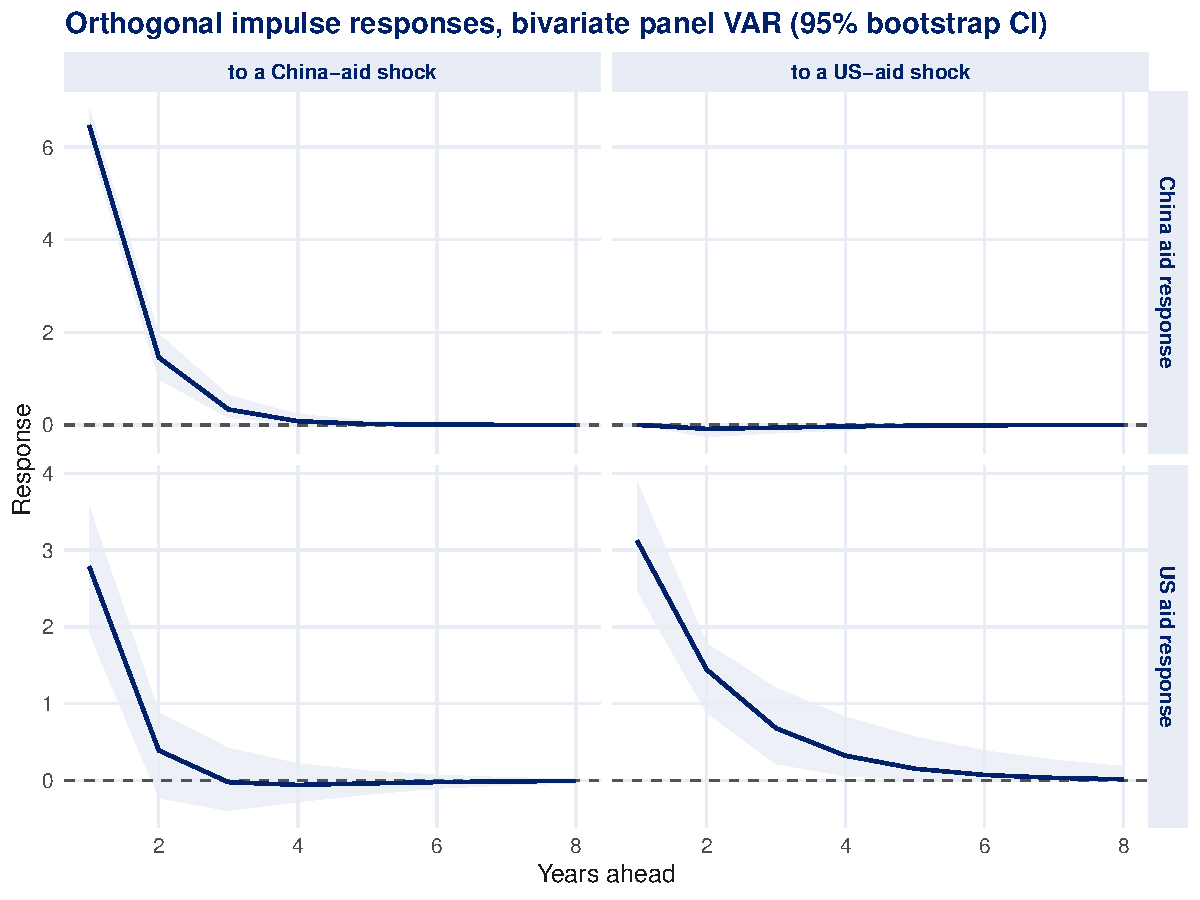
\includegraphics{fig_irf}         %% source: analyses/04_var_dynamics/scripts/R/05_figures.R

\section{Robustness}
\label{sec:quant-robustness}
\textit{Placeholder.} Specification curve / multiverse, leave-one-out by region,
alternative clustering and inference (per the project's inference-robustness
conventions).
.
%
% This chapter carries the dissertation's empirical weight (the qualitative case
% chapters were dropped). Every number here must trace to an R pipeline under
% Dissertation/analyses/NN/. Wiring convention:
%   - Table fragments:  \input{tables/<name>.tex}
%     produced by analyses/01_quant_main/scripts/R/04_tables.R, then copied/
%     written into Dissertation/tables/.
%   - Inline numbers:   annotate with  %% source: analyses/NN/scripts/R/03_analyze.R
%     so /audit-reproducibility can check the paper<->code graph.
% =============================================================================
\chapter{Aid Competition across Spheres of Influence: Quantitative Evidence}
\label{ch:quant}

\textit{Placeholder.} The empirical core. Short-run allocation models by region,
an instrumental-variables strategy for Chinese aid exposure, and a long-run
dynamics test establish whether US and Chinese aid race or diverge across
contested spheres.

\section{Data}
\label{sec:quant-data}
\textit{Placeholder.} AidData Global Chinese Development Finance (GCDF) for
Chinese official finance; OECD-DAC Creditor Reporting System (CRS) for US and
other DAC aid. Unit of analysis: recipient-country $\times$ year. Sample period,
coverage, and the sphere-of-influence covariates defined in
Chapter~\ref{ch:theory}.

\section{Empirical strategy}
\label{sec:quant-strategy}
\textit{Placeholder.} Short-run allocation model with country and year fixed
effects; identification concerns; the Dreher/Zeitz-style shift-share instrument
(Chinese steel production $\times$ recipient exposure) developed in
\texttt{analyses/03\_iv\_robustness/}; and the panel-VAR / Granger test of
long-run co-evolution in \texttt{analyses/04\_var\_dynamics/}.

\section{Results}
\label{sec:quant-results}
\textit{Placeholder.} Main short-run results table:

% \begin{table}[htbp]
\centering
\caption{Short-run US aid response to lagged Chinese finance, by region}
\label{tab:main}
\begin{tabular}{lcc}
\toprule
Region & China (all official finance) & China (ODA-like only) \\
\midrule
Pooled & 0.053*** & 0.046** \\
 & (0.019) & (0.019) \\
 & [N=3300, 150 ctry] & [N=3300, 150 ctry] \\[2pt]
Africa & 0.039 & 0.037 \\
 & (0.038) & (0.035) \\
 & [N=1188, 54 ctry] & [N=1188, 54 ctry] \\[2pt]
Americas & 0.046 & 0.023 \\
 & (0.033) & (0.039) \\
 & [N=770, 35 ctry] & [N=770, 35 ctry] \\[2pt]
Asia & 0.015 & 0.008 \\
 & (0.022) & (0.016) \\
 & [N=858, 39 ctry] & [N=858, 39 ctry] \\[2pt]
Europe & 0.229* & 0.156* \\
 & (0.110) & (0.078) \\
 & [N=242, 11 ctry] & [N=242, 11 ctry] \\[2pt]
Oceania & 0.061 & 0.081 \\
 & (0.067) & (0.075) \\
 & [N=242, 11 ctry] & [N=242, 11 ctry] \\[2pt]
\bottomrule
\end{tabular}
\begin{minipage}{0.9\textwidth}
\vspace{4pt}
\footnotesize Coefficient on log(lagged China finance + 1) from
log(US ODA + 1) $\sim$ log(China finance$_{t-1}$ + 1) with year and
country fixed effects; SEs clustered by country. * p<0.10, ** p<0.05, *** p<0.01.
\end{minipage}
\end{table}
     %% source: analyses/01_quant_main/scripts/R/04_tables.R

\textit{Placeholder.} Report the headline pattern here once the pipeline is run:
a positive US--China aid correlation in Africa
(prospectus: $+0.113$)                                %% source: analyses/01_quant_main/scripts/R/03_analyze.R
and negative correlations outside Africa, consistent with H1.

\section{Instrumental-variables robustness}
\label{sec:quant-iv}
\textit{Placeholder.} IV estimates and first-stage diagnostics:

% \begin{table}[htbp]
\centering
\caption{Shift-share IV for Chinese finance: first-stage diagnostics by share definition}
\label{tab:iv}
\small
\begin{tabular}{lcccc}
\toprule
Exposure share & 1st-stage coef. & 1st-stage $t$ & 1st-stage $F$ & 2SLS estimate \\
\midrule
Predetermined (1970--99) & -0.527 & -0.36 & 0.27 & -2.466 \\
 & & & & (7.648) \\[2pt]
Contemporaneous (2000--15) & 3.089 & 4.97 & 27.33 & 0.321 \\
 & & & & (0.247) \\[2pt]
\bottomrule
\end{tabular}
\begin{minipage}{0.92\textwidth}
\vspace{4pt}
\footnotesize Instrument $=\ln(\text{Chinese crude steel production}_{t-1})\times\text{exposure share}_i$,
following Dreher, Fuchs, Parks, Strange and Tierney (2021). Outcome is $\log(\text{US ODA}+1)$,
endogenous regressor $\log(\text{Chinese official finance}_{t-1}+1)$; year and country fixed
effects, SEs clustered by country. Sample 2000--2015 (bounded by the WSA steel series).
OLS on the same sample: $0.036$**. * p<0.10, ** p<0.05, *** p<0.01.
\textbf{Read this table as a diagnosis, not an estimate.} The predetermined share is the
methodologically valid one and produces no first stage. The contemporaneous share is
constructed from the same post-2000 Chinese-finance variation the instrument is meant to
purge, so its first-stage power is mechanical rather than evidence the design identifies
anything. Neither 2SLS column supports inference.
\end{minipage}
\end{table}
       %% source: analyses/03_iv_robustness/scripts/R/04_tables.R

\section{Long-run dynamics}
\label{sec:quant-var}
\textit{Placeholder.} Panel-VAR impulse responses / Granger-causality:

% \begin{table}[htbp]
\centering
\caption{Bivariate panel VAR: US and Chinese aid, 2000--2021 (system GMM)}
\label{tab:var}
\begin{tabular}{lccc}
\toprule
 & US aid (log, $t-1$) & China aid (log, $t-1$) & Constant \\
\midrule
US aid (log, $t$) & 0.475*** & -0.013 & 8.164*** \\
 & (0.110) & (0.016) & (1.748) \\[2pt]
China aid (log, $t$) & -0.075 & 0.225*** & 9.755*** \\
 & (0.129) & (0.048) & (2.124) \\[2pt]
\bottomrule
\end{tabular}
\begin{minipage}{0.9\textwidth}
\vspace{4pt}
\footnotesize Two-step system GMM, forward-orthogonal-deviations, collapsed
instruments; Windmeijer-corrected SEs in parens. * p<0.10, ** p<0.05, *** p<0.01.
Hansen J test of overidentifying restrictions: $\chi^2(28) = 100.22$, $p < 0.001$ --
\textbf{rejects} at conventional levels (34 instruments over 150 groups); interpret with caution.
Stability: companion-matrix eigenvalues all lie inside the unit circle.
\end{minipage}
\end{table}
      %% source: analyses/04_var_dynamics/scripts/R/04_tables.R
% 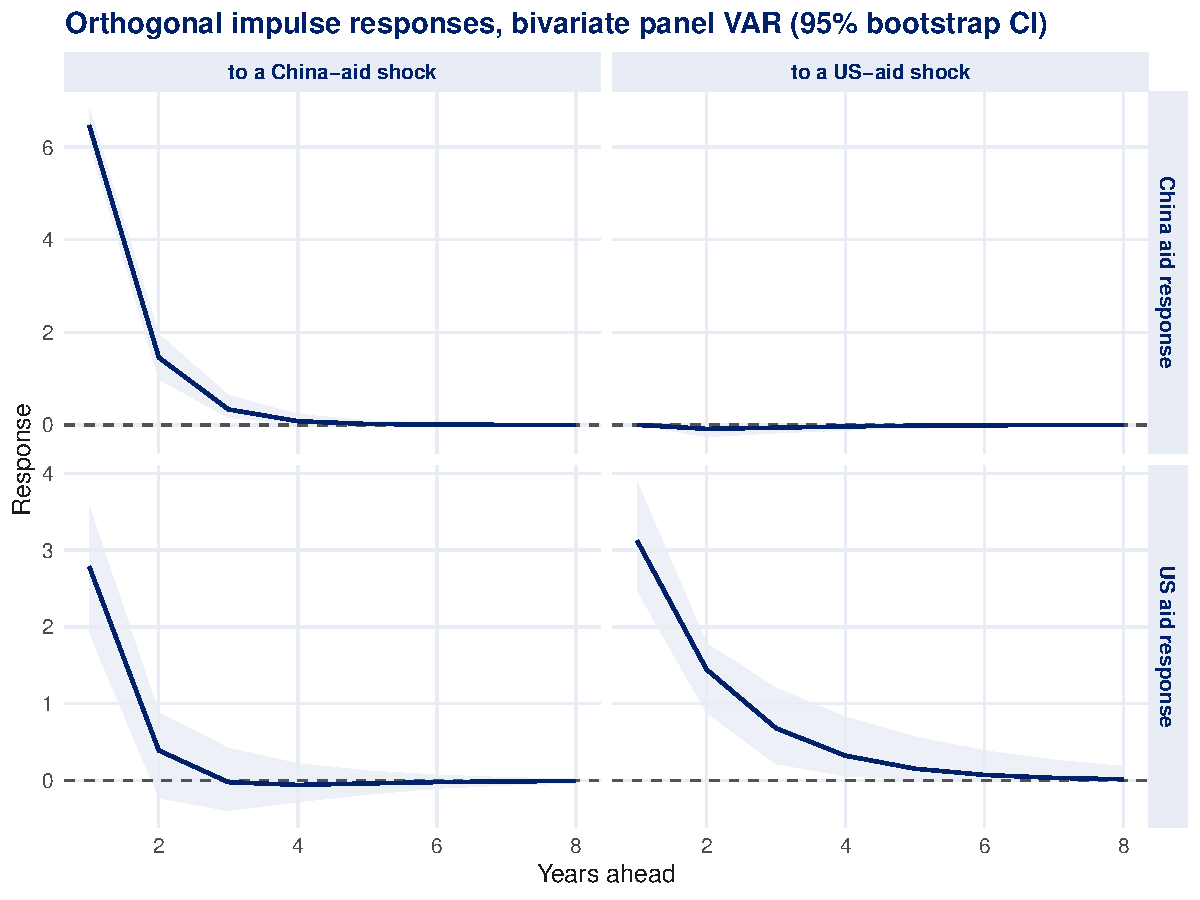
\includegraphics{fig_irf}         %% source: analyses/04_var_dynamics/scripts/R/05_figures.R

\section{Robustness}
\label{sec:quant-robustness}
\textit{Placeholder.} Specification curve / multiverse, leave-one-out by region,
alternative clustering and inference (per the project's inference-robustness
conventions).
.
%
% This chapter carries the dissertation's empirical weight (the qualitative case
% chapters were dropped). Every number here must trace to an R pipeline under
% Dissertation/analyses/NN/. Wiring convention:
%   - Table fragments:  \input{tables/<name>.tex}
%     produced by analyses/01_quant_main/scripts/R/04_tables.R, then copied/
%     written into Dissertation/tables/.
%   - Inline numbers:   annotate with  %% source: analyses/NN/scripts/R/03_analyze.R
%     so /audit-reproducibility can check the paper<->code graph.
% =============================================================================
\chapter{Aid Competition across Spheres of Influence: Quantitative Evidence}
\label{ch:quant}

\textit{Placeholder.} The empirical core. Short-run allocation models by region,
an instrumental-variables strategy for Chinese aid exposure, and a long-run
dynamics test establish whether US and Chinese aid race or diverge across
contested spheres.

\section{Data}
\label{sec:quant-data}
\textit{Placeholder.} AidData Global Chinese Development Finance (GCDF) for
Chinese official finance; OECD-DAC Creditor Reporting System (CRS) for US and
other DAC aid. Unit of analysis: recipient-country $\times$ year. Sample period,
coverage, and the sphere-of-influence covariates defined in
Chapter~\ref{ch:theory}.

\section{Empirical strategy}
\label{sec:quant-strategy}
\textit{Placeholder.} Short-run allocation model with country and year fixed
effects; identification concerns; the Dreher/Zeitz-style shift-share instrument
(Chinese steel production $\times$ recipient exposure) developed in
\texttt{analyses/03\_iv\_robustness/}; and the panel-VAR / Granger test of
long-run co-evolution in \texttt{analyses/04\_var\_dynamics/}.

\section{Results}
\label{sec:quant-results}
\textit{Placeholder.} Main short-run results table:

% \begin{table}[htbp]
\centering
\caption{Short-run US aid response to lagged Chinese finance, by region}
\label{tab:main}
\begin{tabular}{lcc}
\toprule
Region & China (all official finance) & China (ODA-like only) \\
\midrule
Pooled & 0.053*** & 0.046** \\
 & (0.019) & (0.019) \\
 & [N=3300, 150 ctry] & [N=3300, 150 ctry] \\[2pt]
Africa & 0.039 & 0.037 \\
 & (0.038) & (0.035) \\
 & [N=1188, 54 ctry] & [N=1188, 54 ctry] \\[2pt]
Americas & 0.046 & 0.023 \\
 & (0.033) & (0.039) \\
 & [N=770, 35 ctry] & [N=770, 35 ctry] \\[2pt]
Asia & 0.015 & 0.008 \\
 & (0.022) & (0.016) \\
 & [N=858, 39 ctry] & [N=858, 39 ctry] \\[2pt]
Europe & 0.229* & 0.156* \\
 & (0.110) & (0.078) \\
 & [N=242, 11 ctry] & [N=242, 11 ctry] \\[2pt]
Oceania & 0.061 & 0.081 \\
 & (0.067) & (0.075) \\
 & [N=242, 11 ctry] & [N=242, 11 ctry] \\[2pt]
\bottomrule
\end{tabular}
\begin{minipage}{0.9\textwidth}
\vspace{4pt}
\footnotesize Coefficient on log(lagged China finance + 1) from
log(US ODA + 1) $\sim$ log(China finance$_{t-1}$ + 1) with year and
country fixed effects; SEs clustered by country. * p<0.10, ** p<0.05, *** p<0.01.
\end{minipage}
\end{table}
     %% source: analyses/01_quant_main/scripts/R/04_tables.R

\textit{Placeholder.} Report the headline pattern here once the pipeline is run:
a positive US--China aid correlation in Africa
(prospectus: $+0.113$)                                %% source: analyses/01_quant_main/scripts/R/03_analyze.R
and negative correlations outside Africa, consistent with H1.

\section{Instrumental-variables robustness}
\label{sec:quant-iv}
\textit{Placeholder.} IV estimates and first-stage diagnostics:

% \begin{table}[htbp]
\centering
\caption{Shift-share IV for Chinese finance: first-stage diagnostics by share definition}
\label{tab:iv}
\small
\begin{tabular}{lcccc}
\toprule
Exposure share & 1st-stage coef. & 1st-stage $t$ & 1st-stage $F$ & 2SLS estimate \\
\midrule
Predetermined (1970--99) & -0.527 & -0.36 & 0.27 & -2.466 \\
 & & & & (7.648) \\[2pt]
Contemporaneous (2000--15) & 3.089 & 4.97 & 27.33 & 0.321 \\
 & & & & (0.247) \\[2pt]
\bottomrule
\end{tabular}
\begin{minipage}{0.92\textwidth}
\vspace{4pt}
\footnotesize Instrument $=\ln(\text{Chinese crude steel production}_{t-1})\times\text{exposure share}_i$,
following Dreher, Fuchs, Parks, Strange and Tierney (2021). Outcome is $\log(\text{US ODA}+1)$,
endogenous regressor $\log(\text{Chinese official finance}_{t-1}+1)$; year and country fixed
effects, SEs clustered by country. Sample 2000--2015 (bounded by the WSA steel series).
OLS on the same sample: $0.036$**. * p<0.10, ** p<0.05, *** p<0.01.
\textbf{Read this table as a diagnosis, not an estimate.} The predetermined share is the
methodologically valid one and produces no first stage. The contemporaneous share is
constructed from the same post-2000 Chinese-finance variation the instrument is meant to
purge, so its first-stage power is mechanical rather than evidence the design identifies
anything. Neither 2SLS column supports inference.
\end{minipage}
\end{table}
       %% source: analyses/03_iv_robustness/scripts/R/04_tables.R

\section{Long-run dynamics}
\label{sec:quant-var}
\textit{Placeholder.} Panel-VAR impulse responses / Granger-causality:

% \begin{table}[htbp]
\centering
\caption{Bivariate panel VAR: US and Chinese aid, 2000--2021 (system GMM)}
\label{tab:var}
\begin{tabular}{lccc}
\toprule
 & US aid (log, $t-1$) & China aid (log, $t-1$) & Constant \\
\midrule
US aid (log, $t$) & 0.475*** & -0.013 & 8.164*** \\
 & (0.110) & (0.016) & (1.748) \\[2pt]
China aid (log, $t$) & -0.075 & 0.225*** & 9.755*** \\
 & (0.129) & (0.048) & (2.124) \\[2pt]
\bottomrule
\end{tabular}
\begin{minipage}{0.9\textwidth}
\vspace{4pt}
\footnotesize Two-step system GMM, forward-orthogonal-deviations, collapsed
instruments; Windmeijer-corrected SEs in parens. * p<0.10, ** p<0.05, *** p<0.01.
Hansen J test of overidentifying restrictions: $\chi^2(28) = 100.22$, $p < 0.001$ --
\textbf{rejects} at conventional levels (34 instruments over 150 groups); interpret with caution.
Stability: companion-matrix eigenvalues all lie inside the unit circle.
\end{minipage}
\end{table}
      %% source: analyses/04_var_dynamics/scripts/R/04_tables.R
% 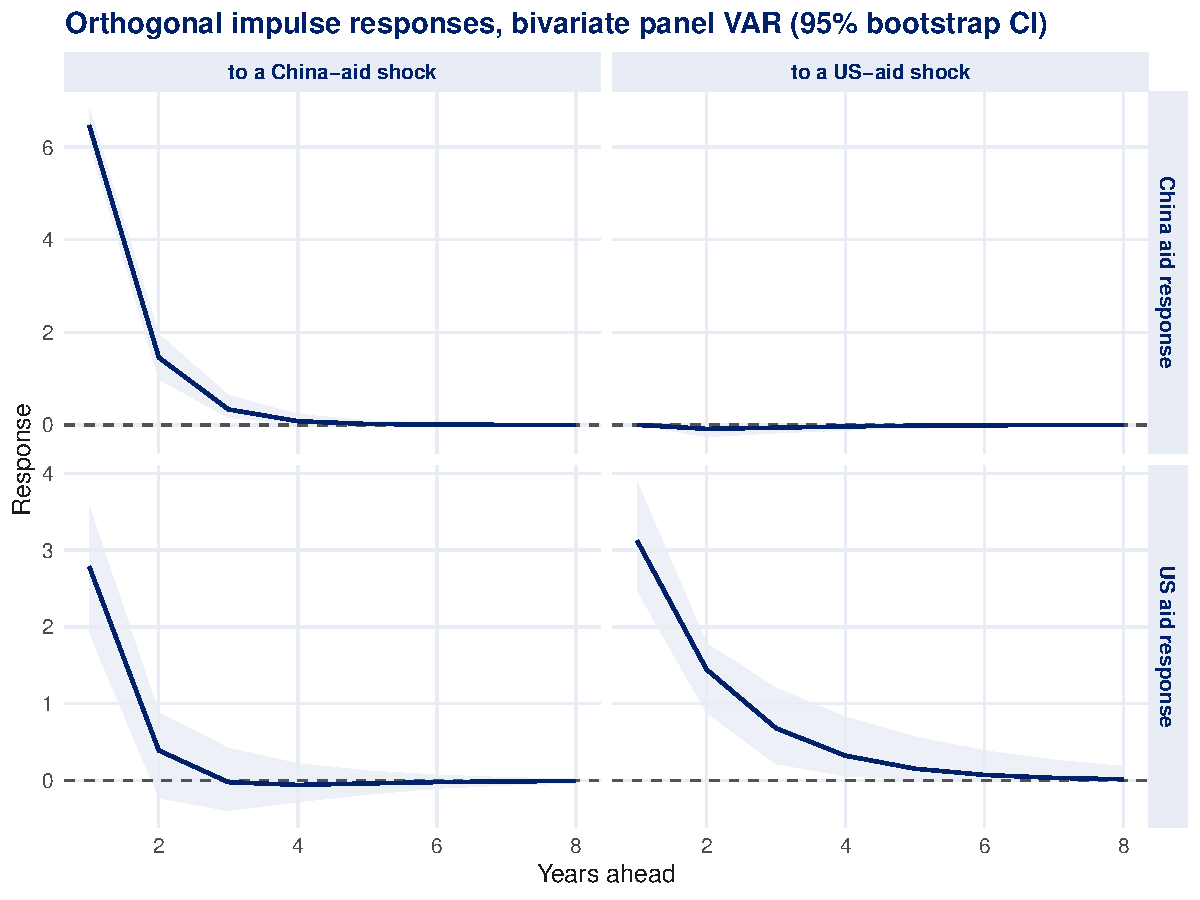
\includegraphics{fig_irf}         %% source: analyses/04_var_dynamics/scripts/R/05_figures.R

\section{Robustness}
\label{sec:quant-robustness}
\textit{Placeholder.} Specification curve / multiverse, leave-one-out by region,
alternative clustering and inference (per the project's inference-robustness
conventions).

% =============================================================================
% chapters/ch05_conclusion.tex — Conclusion
% Pulled into manuscript.tex via % =============================================================================
% chapters/ch05_conclusion.tex — Conclusion
% Pulled into manuscript.tex via % =============================================================================
% chapters/ch05_conclusion.tex — Conclusion
% Pulled into manuscript.tex via \include{chapters/ch05_conclusion}.
% (Was Ch 7 in the Dec 2024 prospectus; renumbered to 5 after the qualitative
%  case-study chapters on Ethiopia, Peru, and Bangladesh were dropped.)
% =============================================================================
\chapter{Conclusion}
\label{ch:conclusion}

\textit{Placeholder.} Restate the argument and what the evidence in
Chapter~\ref{ch:quant} established: where US and Chinese aid race and where the
US withdraws, and how that maps onto contested spheres of influence.

\section{What we learned}
\textit{Placeholder.} The theory survives the data (aid races in Africa, aid
withdrawal elsewhere); the empirical burden the quantitative chapter now carries.

\section{Scope conditions and limitations}
\textit{Placeholder.} External validity, measurement of ``sphere of influence,''
and what the dropped qualitative cases would have added.

\section{Implications and future work}
\textit{Placeholder.} For the aid-competition literature and for policy; and the
parked predict-and-compare reframe (see
\texttt{analyses/05\_advisor\_reframe/SPEC.md}) as a candidate next step.
.
% (Was Ch 7 in the Dec 2024 prospectus; renumbered to 5 after the qualitative
%  case-study chapters on Ethiopia, Peru, and Bangladesh were dropped.)
% =============================================================================
\chapter{Conclusion}
\label{ch:conclusion}

\textit{Placeholder.} Restate the argument and what the evidence in
Chapter~\ref{ch:quant} established: where US and Chinese aid race and where the
US withdraws, and how that maps onto contested spheres of influence.

\section{What we learned}
\textit{Placeholder.} The theory survives the data (aid races in Africa, aid
withdrawal elsewhere); the empirical burden the quantitative chapter now carries.

\section{Scope conditions and limitations}
\textit{Placeholder.} External validity, measurement of ``sphere of influence,''
and what the dropped qualitative cases would have added.

\section{Implications and future work}
\textit{Placeholder.} For the aid-competition literature and for policy; and the
parked predict-and-compare reframe (see
\texttt{analyses/05\_advisor\_reframe/SPEC.md}) as a candidate next step.
.
% (Was Ch 7 in the Dec 2024 prospectus; renumbered to 5 after the qualitative
%  case-study chapters on Ethiopia, Peru, and Bangladesh were dropped.)
% =============================================================================
\chapter{Conclusion}
\label{ch:conclusion}

\textit{Placeholder.} Restate the argument and what the evidence in
Chapter~\ref{ch:quant} established: where US and Chinese aid race and where the
US withdraws, and how that maps onto contested spheres of influence.

\section{What we learned}
\textit{Placeholder.} The theory survives the data (aid races in Africa, aid
withdrawal elsewhere); the empirical burden the quantitative chapter now carries.

\section{Scope conditions and limitations}
\textit{Placeholder.} External validity, measurement of ``sphere of influence,''
and what the dropped qualitative cases would have added.

\section{Implications and future work}
\textit{Placeholder.} For the aid-competition literature and for policy; and the
parked predict-and-compare reframe (see
\texttt{analyses/05\_advisor\_reframe/SPEC.md}) as a candidate next step.


% =============================================================================
% Bibliography. Single shared file at the repo root (../Bibliography_base.bib);
% found via BIBINPUTS=.. at bibtex time. apsr is the political-science default;
% swap to plainnat / apalike if apsr.bst is unavailable in your TeX install.
% =============================================================================
\bibliographystyle{apsr}
\bibliography{../Bibliography_base}

\end{document}
